\section{\label{sec:aufbau}Aufbau}
Der am Versuchstag verwendete Aufbau ist schematisch in Abb.~\ref{fig:aufbau} dargestellt. 
\begin{figure}[h!]
    \centering
    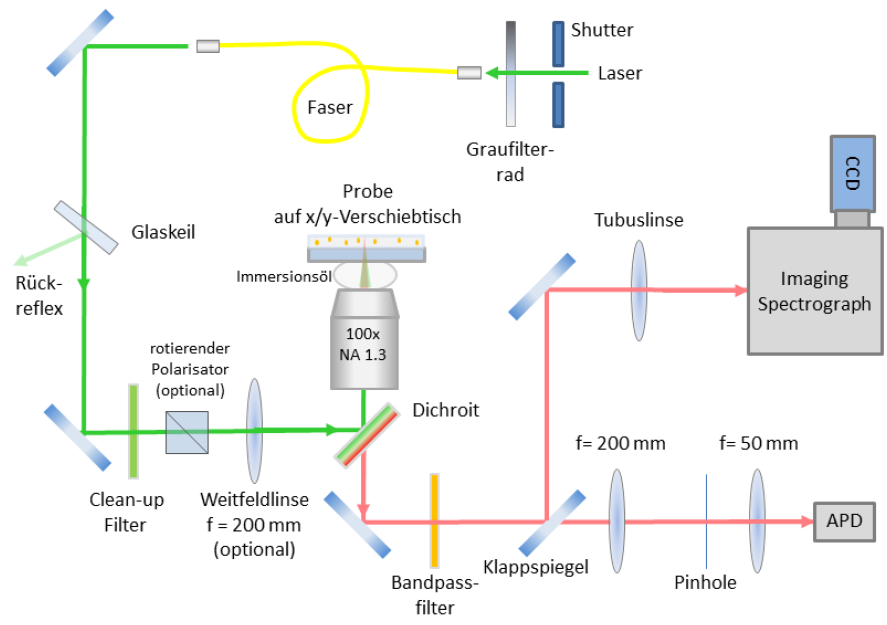
\includegraphics[width=0.7\textwidth]{Versuchsaufbau.png}
    \caption{\label{fig:aufbau}Skizze des Versuchsaufbaus zur Detektion einzelner Moleküle. 
    Die Funktionsweise der einzelnen Komponenten und optionale Variationen sind im Haupttext beschrieben.
    Die Grafik wurde der Anleitung \cite{Anleitung} entnommen.
    Der konfokale Aufbau mit dem Pinhole und der APD (Avalanche Photodiode)
    wird am Versuchstag nicht verwendet.}
\end{figure} \FloatBarrier
Zunächst wird das Laserlicht eines Diodenlasers ($\lambda = 510\,\si{nm}$) über eine Glasfaser 
in den Strahlengang eingekoppelt und über einen Faserpolarisator (nicht eingezeichnet) zirkular polarisert. 
Ein Shutter vor dem Laser ermöglicht es während einer Messpause die Anregungszeit der
Probe zu reduzieren, um das Ausbleichen der Moleküle zu vermeiden. Zudem kann die Anregungsleistung über Graufilterrad 
eingestellt werden. Über Spiegel wird der Strahl auf den dichroitischen Filter geleitet, welcher für verschiedene 
Wellenlänge reflektierend oder transmittierend wirkt (vgl.~Abschnitt \ref{subsec:FZV6}). Der Filter ist so gewählt,
dass das energiereichere Anregungslicht in das Mikroskopobjektiv reflektiert wird, wo es auf die Probe 
fokussiert, welche auf einem verschiebbaren Tisch befestigt ist. Das von der Probe emittierte energieärmere 
Fluoreszenzlicht wird vom Filter durchgelassen. 
Der Clean-up Filter im vorderen Strahlengang unterdrückt unerwünschte Störsignale der optischen Bauteile, während 
der Glaskeil als Kontrollelement für die Fokussierung der Probe genutzt wird. \\
Nach Transmission durch den dichroitischen Filter wird der Strahl über Spiegel in den Spektrographen geleitet. 
Ein Bandpassfilter säubert das Fluoreszenzlicht nochmals von restlichem Anregungslicht, um das Signal-Rausch-Verhältnis 
zu optimieren. Durch die Tubuslinse im Strahlengang ist das Mikroskop vollständig und das vergrößerte Bild 
gelangt in den Spektrographen, welcher wahlweise ein Gitter (150 Linien/mm) oder einen Spiegel in den Strahlengang 
beifügt. Das Signal wird über eine Einzelphotonen-empfindliche CCD Kamera gemessen, die für den Versuch mit 
2x2-Binning betrieben wird (vgl.~Abschnitt \ref{subsec:FZV10}). \\ 
Der Versuchsaufbau lässt sich durch optionale Bauteile variieren. 
Wird die Weitfeldlinse in den Strahlengang geklappt, so kann die Probe großflächig angeregt werden und das 
Signal über den Spektrographen im Spiegelmodus auf die CCD-Kamera geleitet werden. Hierzu muss der 
Spalt weit geöffnet sein. Will man die Spektren der einzelnen Moleküle aufnehmen, so muss das Gitter 
im Spektrographen eingestellt. Außerdem wird die Weitfeldlinse entfernt, wodurch 
sich das angeregte Probenvolumen verkleinert. \\ 
Für die Polarisationsabhängige Messung kann ein rotierender Polarisator eingebracht werden. Zudem lässt sich 
die Anregungsleistung über ein einklappbares Powermeter (nicht eingezeichnet) bestimmen, welches 
vor der Weitfeldlinse im Strahlengang platziert werden kann. \\
Die Durchführungsschritte der einzelnen Versuchsteile, sowie die Präsentationen und Analysen der 
Ergebnisse werden im nächsten Abschnitt beschrieben. \\


